\documentclass[../../main/main.tex]{subfiles}

\begin{document}



% \newcommand{\JetsZero}{../../plots/pdf/Jets06/0.902_500_1000_1.0_1e-05_06-01-1046}
% \newcommand{\JetsOne}{../../plots/pdf/Jets06/0.902_500_1000_1.0_1e-05_06-01-1046}
\newcommand{\FillMean}{../../plots/pdf/FillMean6/0.915_0.607_500_1000_1.0_0.0001}
\newcommand{\FillZero}{../../plots/pdf/FillZero6/0.913_0.647_500_1000_1.0_1e-06}
\newcommand{\FillPhiRandom}{../../plots/pdf/FillPhiRandom6/0.915_0.607_500_1000_1.0_0.0001}
\newcommand{\RemoveJets}{../../plots/pdf/RemoveJets6/0.908_0.526_500_1000_1.0_1e-05}
\newcommand{\RemovePhi}{../../plots/pdf/RemovePhi6/0.915_0.567_500_1000_1.0_0.0001}
\newcommand{\JetsNone}{../../plots/pdf/Jets06/0.902_0.405_500_1000_1.0_1e-05}
\newcommand{\JetsOne}{../../plots/pdf/Jets16/0.895_0.647_500_1000_1.0_0.0001}
\newcommand{\JetsTwo}{../../plots/pdf/Jets26/0.932_0.97_500_1000_1.0_1e-05}

\newcommand{\captionAcc}{Train (blue) and test (orange) accuracy.}
\newcommand{\captionLoss}{Train (blue) and test (orange) loss.}
\newcommand{\captionROC}{ROC curve of the neural network output.}
\newcommand{\captionDataset}[1]{The accuracy (a), loss (b) and the ROC curve (c) of the neural network output from the \emph{#1} dataset with \(\lambda=1\) and \(\eta=0.0001\).}
\newcommand{\captionBkgSig}{dd}
\newcommand{\captionLik}{dd}
\newcommand{\captionDatasetZ}[1]{#1}

\section{Results}
\label{sec:results}

The results that follows are obtained from a grid search where we present best results with the accuracy in a grid with the values of the learning rate \(\lambda\in[.....]\) and \(\eta\in [1,10^{-1},10^{-2},10^{-3},10^{-5}]\) . The other results from the grid search can be found in the GitHub repository\footnote{test}. I all of the training of the neural networks for the different datasets explained in Section \ref{sec:missing-variables} we use a batch size of 50 000 and train it for 500 epochs.


\subsection{FillMean dataset}
\label{sec:fillmean-dataset}


Figure \ref{fig:FillMean_1} shows the output from the neural network with the dataset \emph{FillMean} described in Section \ref{sec:inserting-values} with the accuracy in Figure \ref{fig:FillMean_acc}, loss in Figure \ref{fig:FillMean_loss} and the ROC curve in Figure \ref{fig:FillMean_roc}. The values for the hyperparameters that gave the best results for the neural network from the grid search are \(\eta=1\) and \(\lambda=0.0001\). We see that for both the accuracy and the loss from the training and test data are similar to each other respectively indicating that there is little over training. In addition the accuracy is stable over the epochs while the loss seems to approach a minimum. This indicates that the neural network has learned much of what it can learn from the dataset. The accuracy of the training dataset is 0.844 after the 500th epcoh, while the area under the ROC curve (AUC) in Figure \ref{fig:FillMean_roc} is 0.915.

Figure \ref{fig:FillMean_Z} shows the distribution of the true background and signal events over the output from the neural network in Figure \ref{fig:FillMean_bkg_sig} and the log-likelihood ratio of the signal + background and the background estimation \(t(\mu)\) in Figure \ref{fig:FillMean_bkg_sig} which is shifted by the minimum of \(t(\mu)\) with \(t(\mu_{min})\). We observe that the distribution of the true background and signal events in Figure \ref{fig:FillMean_bkg_sig} are mostly skewed towards 0 and 1 respectively which tells us that most of the events in the dataset has been correctly classified. To calculate the \(Z\) score we do a cut at 0.9 as shown by the green dashed line Figure \ref{fig:fillmean_bkgsig}. Counting the background and signal events above 0.9 gives and using Eq. ... gives us \(Z=...\). The estimated likelihood ratio from the neural network is used to find the
 In Figure \ref{fig:FillMean_bkg_sig} we do a cut at 0.9 and obtain \(Z_{cut} = 282.852\) when we have used Eq. ... with the number of background and signal events above 0.9 in Figure \ref{fig:FillMean_bkg_sig}. From Figure \ref{fig:FillMean_likelihood} we get the \(Z_{likelihood} = 429.963\) by using Eq. ... when \(\mu_{min} = 0.607\). The \(\mu\) value where \(t(\mu)\) has it minimum is not at \(\mu=1\) which would be expected from the signal + background hypotosis, and therefore indicates that the neural network has not learned the profile likelihood ratio correctly. The condition for the likelihood ratio estimation from Section \ref{sec:likel-estim} was that the loss function should reach a minima in the training, and Figure \ref{fig:FillMean_loss} shows that the loss function seems to reach a minima, but it that it has not converged to one.

% \newpage


\begin{figure}[H]
  \centering
  \begin{subfigure}[t]{0.5\textwidth}
    \centering
    \includegraphics[width = 1\linewidth]{\FillMean/accuracy.pdf}
    \caption{\captionAcc}
    \label{fig:FillMean_acc}
  \end{subfigure}
  \vspace{0.01cm}
  \begin{subfigure}[t]{0.5\textwidth}
    \centering
    \includegraphics[width = 1\linewidth]{\FillMean/loss.pdf}
    \caption{\captionLoss}
    \label{fig:FillMean_loss}
  \end{subfigure}
  \begin{subfigure}[t]{0.5\textwidth}
    \centering
    \includegraphics[width = 1\linewidth]{\FillMean/roc.pdf}
    \caption{\captionROC}
    \label{fig:FillMean_roc}
  \end{subfigure}
  \caption{\captionDataset{FillMean}}
  \label{fig:FillMean_1}  
\end{figure}

\begin{figure}[H]
  \centering
  \begin{subfigure}[t]{0.5\textwidth}
    \centering
    \includegraphics[width = 1\linewidth]{\FillMean/bkg_sig.pdf}
    \caption{\captionBkgSig}    
    \label{fig:FillMean_bkg_sig}
  \end{subfigure}
  \vspace{0.01cm}
  \begin{subfigure}[t]{0.5\textwidth}
    \centering
    \includegraphics[width = 1\linewidth]{\FillMean/likelihood.pdf}
    \caption{\captionLik}    
    \caption{}
    \label{fig:FillMean_likelihood}
  \end{subfigure}
  \caption{\captionDatasetZ{FillMean}}
  \label{fig:FillMean_Z}
\end{figure}

\subsection{FillZero}
\label{sec:fillzero}

Figure \ref{fig:FillZero_1} shows the output from the neural network with the dataset \emph{FillMean} described in Section \ref{sec:inserting-values} where missing entries are filled with zero and shows the accuracy in Figure \ref{fig:FillZero_acc}, loss in Figure \ref{fig:FillZero_loss} and the ROC curve in Figure \ref{fig:FillZero_roc}. The values for the hyperparameters that gave the best results for the neural network from the grid search are \(\eta=1\) and \(\lambda=10^{-6}\). We see that there is a descrepancy between the values from the training and the testing for both the accuracy and the loss where the accuracy and loss becomes stable for the test dataset, while the accuracy contunies grow and the loss continues to decrease for the training dataset. This can be a sign of the model starting to overfitt the data. The accuracy of the training dataset is 0.839 after the 500th epcoh, while the AUC in Figure \ref{fig:FillZero_roc} is 0.913. Filling the missing entries with zero in particle physics is always not physical since objects, like a jet that is missing would not have any momentum or a direction, and it would therefore cause a bias by inserting a value in the dataset, even if it is zero.

Figure \ref{fig:FillZero_Z} shows the distribution of the true background and signal events over the output from the neural network in Figure \ref{fig:FillZero_bkg_sig}, and the log-likelihood ratio of the signal + background and the background estimation \(t(\mu)\) in Figure \ref{fig:FillZero_bkg_sig}. We observe that the distribution of the true background and signal events in Figure \ref{fig:FillZero_bkg_sig} are mostly skewed towards 0 and 1 respectively which tells us that most of the events in the dataset has been correctly classified. In Figure \ref{fig:FillZero_bkg_sig} we do a cut at 0.9 and obtain \(Z_{cut} = 290.612\) when we have used Eq. ... with the number of background and signal events above 0.9 in Figure \ref{fig:FillZero_bkg_sig}. The log-likelihood function in Figure \ref{fig:FillZero_likelihood}  shifted by the minimum of \(t(\mu)\), \(t(\mu_{min})\), where the minima of the log-likelihood is located at \(\mu_{min} = 0.647\). The minima is not located at \(\mu=1\) which is the expected signal strength under the signal+background hypothosi, and this indicates that the neural network has not learned the likelihood ratio from from the dataset correctly. By using Eq. ..., the \(Z_{likelihood}\) is found to be \(Z_{likelihood} = 483.050\). The condition for the likelihood ratio estimation from Section \ref{sec:likel-estim} was that the loss function should reach a minima in the training, and Figure \ref{fig:FillZero_loss} shows that the loss function seems to reach a minima, but it that it has not converged to one.




\begin{figure}[H]
  \centering
  \begin{subfigure}[t]{0.5\textwidth}
    \centering
    \includegraphics[width = 1\linewidth]{\FillZero/accuracy.pdf}
    \caption{\captionAcc}
    \label{fig:FillZero_acc}
  \end{subfigure}
  \vspace{0.01cm}
  \begin{subfigure}[t]{0.5\textwidth}
    \centering
    \includegraphics[width = 1\linewidth]{\FillZero/loss.pdf}
    \caption{\captionLoss}
    \label{fig:FillZero_loss}
  \end{subfigure}
  \begin{subfigure}[t]{0.5\textwidth}
    \centering
    \includegraphics[width = 1\linewidth]{\FillZero/roc.pdf}
    \caption{\captionROC}
    \label{fig:FillZero_roc}
  \end{subfigure}
  \caption{\captionDataset{FillZero}}
  \label{fig:FillZero_1}  
\end{figure}

\begin{figure}[H]
  \centering
  \begin{subfigure}[t]{0.5\textwidth}
    \centering
    \includegraphics[width = 1\linewidth]{\FillZero/bkg_sig.pdf}
    \caption{\captionBkgSig}    
    \label{fig:FillZero_bkg_sig}
  \end{subfigure}
  \vspace{0.01cm}
  \begin{subfigure}[t]{0.5\textwidth}
    \centering
    \includegraphics[width = 1\linewidth]{\FillZero/likelihood.pdf}
    \caption{\captionLik}    
    \label{fig:FillZero_likelihood}
  \end{subfigure}
  \caption{\captionDatasetZ{FillZero}}
  \label{fig:FillZero_Z}
\end{figure}

\subsection{FillPhiRandom}
\label{sec:fillzero}
% where the missing in the \(\phi\) variables are filled with random variables between \(-\pi\) and \(\pi\), and the other missing entries are filled with the mean of the corresponding variable.
The results from the neural network for the \emph{FillPhiRandom} dataset described in Section \ref{sec:inserting-values} are shown in Figure \ref{fig:FillPhiRandom_1} where Figure \ref{fig:FillPhiRandom_acc} shows the accuracy, Figure \ref{fig:FillPhiRandom_loss} shows the loss, and Figure \ref{fig:FillZero_roc} shows the ROC curve. The values for the hyperparameters that gave the best results for the neural network from the grid search are \(\eta=1\) and \(\lambda=0.0001\). When we compare these results with the ones from the \emph{FillMean} dataset we see that they are almost identical. Both the accuracy and the loss follows the same shape, and the training and testing results are almost the same. The accuracy of the training dataset is 0.845 after the 500th epcoh, while the AUC in Figure \ref{fig:FillPhiRandom_roc} is 0.915, which also are almost identical to the results from the \emph{FillMean} dataset. The fact that the results from the training on the \emph{FillMean} and \emph{FillPhiRandom} datasets almost gives the same reslults can be undersood from the fact that the only varialbes that have different values between them is the \(\phi\) variables which are almost uniform as shown in Figure ... in Appendix. This means that filling the missing entries with the mean of that variable or a random number between \(-\pi\) and \(\pi\) indicated that the \(\phi\) feautures are not of high importance compared to the other features that the datasets include. From a physics view (if time).


\begin{figure}[H]
  \centering
  \begin{subfigure}[t]{0.5\textwidth}
    \centering
    \includegraphics[width = 1\linewidth]{\FillPhiRandom/accuracy.pdf}
    \caption{\captionAcc}
    \label{fig:FillPhiRandom_acc}
  \end{subfigure}
  \vspace{0.01cm}
  \begin{subfigure}[t]{0.5\textwidth}
    \centering
    \includegraphics[width = 1\linewidth]{\FillPhiRandom/loss.pdf}
    \caption{\captionLoss}
    \label{fig:FillPhiRandom_loss}
  \end{subfigure}
  \begin{subfigure}[t]{0.5\textwidth}
    \centering
    \includegraphics[width = 1\linewidth]{\FillPhiRandom/roc.pdf}
    \caption{\captionROC}
    \label{fig:FillPhiRandom_roc}
  \end{subfigure}
  \caption{\captionDataset{FillPhiRandom}}
  \label{fig:FillPhiRandom_1}  
\end{figure}

\begin{figure}[H]
  \centering
  \begin{subfigure}[t]{0.5\textwidth}
    \centering
    \includegraphics[width = 1\linewidth]{\FillPhiRandom/bkg_sig.pdf}
    \caption{\captionBkgSig}    
    \label{fig:FillPhiRandom_bkg_sig}
  \end{subfigure}
  \vspace{0.01cm}
  \begin{subfigure}[t]{0.5\textwidth}
    \centering
    \includegraphics[width = 1\linewidth]{\FillPhiRandom/likelihood.pdf}
    \caption{\captionLik}    
    \label{fig:FillPhiRandom_likelihood}
  \end{subfigure}
  \caption{\captionDatasetZ{FillPhiRandom}}
  \label{fig:FillPhiRandom_Z}
\end{figure}


\subsection{RemovePhi}
\label{sec:removephi}

For the dataset \emph{RemovePhi} where we remove the \(\phi\) angle features the results of the neural network are shown in Figure \ref{fig:RemovePhi_acc} with the accuracy in Figure \ref{fig:RemovePhi_acc}, loss in Figure \ref{fig:RemovePhi_loss} and the ROC curve in Figure \ref{fig:RemoveJets_roc}. The values for the hyperparameters that gave the best results for the neural network from the grid search are \(\eta=1\) and \(\lambda=0.0001\), similar to the training on the \emph{FillMean} and \emph{FillPhirandom} datasets. In this case as well the results from the accuracy, loss and ROC curve are similar to the results for the \emph{FillMean} and \emph{FillPhiRandom} datasets, and accuracy of the training dataset is 0.844 after the 500th epcoh, while the area under the ROC curve (AUC) in Figure \ref{fig:FillMean_roc} is 0.915. This gives us another inducation that the \(\phi\) features are not important for the training since the results are the almost the same when we include them in the dataset.  We see that for both the accuracy and the loss from the training and test data are similar to each other respectively indicating that there is little over training. In addition the accuracy is stable over the epochs while the loss seems to approach a minimum. This indicates that the neural network has learned much of what it can learn from the dataset. The accuracy of the training dataset is 0.844 after the 500th epcoh, while the area under the ROC curve (AUC) in Figure \ref{fig:FillMean_roc} is 0.915.




\begin{figure}[H]
  \centering
  \begin{subfigure}[t]{0.5\textwidth}
    \centering
    \includegraphics[width = 1\linewidth]{\RemovePhi/accuracy.pdf}
    \caption{\captionAcc}
    \label{fig:RemovePhi_acc}
  \end{subfigure}
  \vspace{0.01cm}
  \begin{subfigure}[t]{0.5\textwidth}
    \centering
    \includegraphics[width = 1\linewidth]{\RemovePhi/loss.pdf}
    \caption{\captionLoss}
    \label{fig:RemovePhi_loss}
  \end{subfigure}
  \begin{subfigure}[t]{0.5\textwidth}
    \centering
    \includegraphics[width = 1\linewidth]{\RemovePhi/roc.pdf}
    \caption{\captionROC}
    \label{fig:RemovePhi_roc}
  \end{subfigure}
  \caption{\captionDataset{RemovePhi}}
  \label{fig:RemovePhi_1}  
\end{figure}

\begin{figure}[H]
  \centering
  \begin{subfigure}[t]{0.5\textwidth}
    \centering
    \includegraphics[width = 1\linewidth]{\RemovePhi/bkg_sig.pdf}
    \caption{\captionBkgSig}    
    \label{fig:RemovePhi_bkg_sig}
  \end{subfigure}
  \vspace{0.01cm}
  \begin{subfigure}[t]{0.5\textwidth}
    \centering
    \includegraphics[width = 1\linewidth]{\RemovePhi/likelihood.pdf}
    \caption{\captionLik}    
    \label{fig:RemovePhi_likelihood}
  \end{subfigure}
  \caption{\captionDatasetZ{RemovePhi}}
  \label{fig:RemovePhi_Z}
\end{figure}

\subsection{RemoveJets}
\label{sec:fillzero}

Figure \ref{fig:RemoveJets_1} shows the output from the neural network with the dataset \emph{RemoveJets} described in Section \ref{sec:inserting-values} where we remove the jets feautures, with the accuracy in Figure \ref{fig:RemoveJets_acc}, loss in Figure \ref{fig:RemoveJets_loss} and the ROC curve in Figure \ref{fig:RemoveJets_roc}. The values for the hyperparameters that gave the best results for the neural network from the grid search are \(\eta=1\) and \(\lambda=0.0001\). We see that for both the accuracy and the loss from the training and test data are similar to each other respectively indicating that there is little over training, but that there are a small descrepancy between them. In addittion to this the accuracy and loss converges to a value which indicates that the model has learned what it can from the dataset. That it converges faster than for e.g \emph{FillMean} comes from the fact that it has fewer input feauters which leads to less information. This shows that in this case it is not an advantage to remove feautures that has missing variables. If the variables had a larger fraction of missing entries then it would maybe advatougus to remove these feautures since any filling of these variables might lead to more noise in the dataset. In addition the accuracy is stable over the epochs while the loss seems to approach a minimum. This indicates that the neural network has learned much of what it can learn from the dataset. The accuracy of the training dataset is 0.844 after the 500th epcoh, while the area under the ROC curve (AUC) in Figure \ref{fig:FillMean_roc} is 0.915.

\begin{figure}[H]
  \centering
  \begin{subfigure}[t]{0.5\textwidth}
    \centering
    \includegraphics[width = 1\linewidth]{\RemoveJets/accuracy.pdf}
    \caption{\captionAcc}
    \label{fig:RemoveJets_acc}
  \end{subfigure}
  \vspace{0.01cm}
  \begin{subfigure}[t]{0.5\textwidth}
    \centering
    \includegraphics[width = 1\linewidth]{\RemoveJets/loss.pdf}
    \caption{\captionLoss}
    \label{fig:RemoveJets_loss}
  \end{subfigure}
  \begin{subfigure}[t]{0.5\textwidth}
    \centering
    \includegraphics[width = 1\linewidth]{\RemoveJets/roc.pdf}
    \caption{\captionROC}
    \label{fig:RemoveJets_roc}
  \end{subfigure}
  \caption{\captionDataset{RemoveJets}}
  \label{fig:RemoveJets_1}  
\end{figure}

\begin{figure}[H]
  \centering
  \begin{subfigure}[t]{0.5\textwidth}
    \centering
    \includegraphics[width = 1\linewidth]{\RemoveJets/bkg_sig.pdf}
    \caption{\captionBkgSig}    
    \label{fig:RemoveJets_bkg_sig}
  \end{subfigure}
  \vspace{0.01cm}
  \begin{subfigure}[t]{0.5\textwidth}
    \centering
    \includegraphics[width = 1\linewidth]{\RemoveJets/likelihood.pdf}
    \caption{\captionLik}    
    \label{fig:RemoveJets_likelihood}
  \end{subfigure}
  \caption{\captionDatasetZ{RemoveJets}}
  \label{fig:RemoveJets_Z}
\end{figure}

\subsection{JetsNone}
\label{sec:fillzero}


\begin{figure}[H]
  \centering
  \begin{subfigure}[t]{0.5\textwidth}
    \centering
    \includegraphics[width = 1\linewidth]{\JetsNone/accuracy.pdf}
    \caption{\captionAcc}
    \label{fig:JetsNone_acc}
  \end{subfigure}
  \vspace{0.01cm}
  \begin{subfigure}[t]{0.5\textwidth}
    \centering
    \includegraphics[width = 1\linewidth]{\JetsNone/loss.pdf}
    \caption{\captionLoss}
    \label{fig:JetsNone_loss}
  \end{subfigure}
  \begin{subfigure}[t]{0.5\textwidth}
    \centering
    \includegraphics[width = 1\linewidth]{\JetsNone/roc.pdf}
    \caption{\captionROC}
    \label{fig:JetsNone_roc}
  \end{subfigure}
  \caption{\captionDataset{JetsNone}}
  \label{fig:JetsNone_1}  
\end{figure}

\begin{figure}[H]
  \centering
  \begin{subfigure}[t]{0.5\textwidth}
    \centering
    \includegraphics[width = 1\linewidth]{\JetsNone/bkg_sig.pdf}
    \caption{\captionBkgSig}    
    \label{fig:JetsNone_bkg_sig}
  \end{subfigure}
  \vspace{0.01cm}
  \begin{subfigure}[t]{0.5\textwidth}
    \centering
    \includegraphics[width = 1\linewidth]{\JetsNone/likelihood.pdf}
    \caption{\captionLik}    
    \label{fig:JetsNone_likelihood}
  \end{subfigure}
  \caption{\captionDatasetZ{JetsNone}}
  \label{fig:JetsNone_Z}
\end{figure}

\subsection{JetsOne}
\label{sec:fillzero}


\begin{figure}[H]
  \centering
  \begin{subfigure}[t]{0.5\textwidth}
    \centering
    \includegraphics[width = 1\linewidth]{\JetsOne/accuracy.pdf}
    \caption{\captionAcc}
    \label{fig:JetsOne_acc}
  \end{subfigure}
  \vspace{0.01cm}
  \begin{subfigure}[t]{0.5\textwidth}
    \centering
    \includegraphics[width = 1\linewidth]{\JetsOne/loss.pdf}
    \caption{\captionLoss}
    \label{fig:JetsOne_loss}
  \end{subfigure}
  \begin{subfigure}[t]{0.5\textwidth}
    \centering
    \includegraphics[width = 1\linewidth]{\JetsOne/roc.pdf}
    \caption{\captionROC}
    \label{fig:JetsOne_roc}
  \end{subfigure}
  \caption{\captionDataset{JetsOne}}
  \label{fig:JetsOne_1}  
\end{figure}

\begin{figure}[H]
  \centering
  \begin{subfigure}[t]{0.5\textwidth}
    \centering
    \includegraphics[width = 1\linewidth]{\JetsOne/bkg_sig.pdf}
    \caption{\captionBkgSig}    
    \label{fig:JetsOne_bkg_sig}
  \end{subfigure}
  \vspace{0.01cm}
  \begin{subfigure}[t]{0.5\textwidth}
    \centering
    \includegraphics[width = 1\linewidth]{\JetsOne/likelihood.pdf}
    \caption{\captionLik}    
    \label{fig:JetsOne_likelihood}
  \end{subfigure}
  \caption{\captionDatasetZ{JetsOne}}
  \label{fig:JetsOne_Z}
\end{figure}

\subsection{JetsTwo}
\label{sec:fillzero}


\begin{figure}[H]
  \centering
  \begin{subfigure}[t]{0.5\textwidth}
    \centering
    \includegraphics[width = 1\linewidth]{\JetsTwo/accuracy.pdf}
    \caption{\captionAcc}
    \label{fig:JetsTwo_acc}
  \end{subfigure}
  \vspace{0.01cm}
  \begin{subfigure}[t]{0.5\textwidth}
    \centering
    \includegraphics[width = 1\linewidth]{\JetsTwo/loss.pdf}
    \caption{\captionLoss}
    \label{fig:JetsTwo_loss}
  \end{subfigure}
  \begin{subfigure}[t]{0.5\textwidth}
    \centering
    \includegraphics[width = 1\linewidth]{\JetsTwo/roc.pdf}
    \caption{\captionROC}
    \label{fig:JetsTwo_roc}
  \end{subfigure}
  \caption{\captionDataset{JetsTwo}}
  \label{fig:JetsTwo_1}  
\end{figure}

\begin{figure}[H]
  \centering
  \begin{subfigure}[t]{0.5\textwidth}
    \centering
    \includegraphics[width = 1\linewidth]{\JetsTwo/bkg_sig.pdf}
    \caption{\captionBkgSig}    
    \label{fig:JetsTwo_bkg_sig}
  \end{subfigure}
  \vspace{0.01cm}
  \begin{subfigure}[t]{0.5\textwidth}
    \centering
    \includegraphics[width = 1\linewidth]{\JetsTwo/likelihood.pdf}
    \caption{\captionLik}    
    \label{fig:JetsTwo_likelihood}
  \end{subfigure}
  \caption{\captionDatasetZ{JetsTwo}}
  \label{fig:JetsTwo_Z}
\end{figure}

To compare and summarize the results we see that among the datasets \emph{FillMean}, \emph{FillZero} and \emph{FillPhiRandom}, both \emph{FillMean} and \emph{FillPhiRandom} gives similar results when we look at the accuracy, loss and the AUC. In the case of \emph{FillZero} it distingushes from the others that it learns the dataset faster and gives a lower AUC compared to the \emph{FillMean} and the \emph{FillPhiRandom} datasets.

When we compare the results from the two datasets \emph{RemovePhi} and \emph{FillMean} we observe that removing the \(\phi\) feautures does not influence the results from the training compared with \emph{FillMean} where we keep the \(\phi\) feautures. This tells us that the \(\phi\) feautures are not among the most important feautures of the Higgs dataset.

In the case of the dataset \emph{RemoveJets} when we have removed the feautures that has missing entries (except MMHiggs) we get a lower performance of the trained model compared to \emph{FillMean} which indicates that the neural network learns from the jet feautures in the dataset and is not influenced to much by the noise when inserting the mean in the dataset. The best result with the accuracy was for the \emph{Jets2} dataset which had the most features among \emph{Jets0}, \emph{Jets1} and \emph{Jets2}, and was also the dataset that was the most balanced with background and signal events. However it did not have the best discovery significanse since it had less statistics than e.g \emph{FillMean}. But the likelihood estimation gave the profile likelihood function that had \(\hat{\mu}=0.97\) which was closest to the expected signal strength equal to 1 indicating that it learned the likelhood ratio better than for the other datasets.

\begin{table}[H]
 \caption{Summary of the results for the different datasets
 }
    \label{tab:acronyms}
  \centering
  \begin{ruledtabular}
  \begin{tabular}{l|lllll}
    Dataset & accuracy & AUC & \(Z_{cut}\) & \(Z_{likelihood}\) & \(\mu_{min}\)\\
    \hline
    \emph{FillMean} & 0.844 & 0.915 & 282.852 & 429.963 & 0.607 \\
    \emph{FillZero} & 0.839 & 0.913 & 290.612 & 483.050 & 0.647 \\
    \emph{FillPhiRandom} & 0.838 & 0.908 & 282.852 & 429.963 & 0.607 \\
    \hline
    \emph{RemoveJets} & 0 & 0.908 & 282.852 & 429.963 & 0.526 \\
    \emph{RemovePhi} & 0 & 0.915 & 282.852 & 429.963 & 0.567 \\
    \hline
    \emph{JetsNone} & 0 & 0.902 & 282.852 & 429.963 & 0.405 \\
    \emph{JetsOne} & 0 & 0.895 & 282.852 & 429.963 & 0.647 \\
    \emph{JetsTwo} & 0 & 0.932 & 282.852 & 429.963 & 0.970 \\                        
    
  \end{tabular}
  \end{ruledtabular}
\end{table}

\section{Conclusion}
\label{sec:conclusion}

We have in this project tested various ways of handling the HiggsML dataset which are used to train a neural network, and the output is used to calculate the discovery significanse by using a search region and via likelhood estimation. The dataset that gave the highest discovery significance was the \emph{FillMean} dataset which gave \(Z=429.963\) from the likelhood estimation. However, the \emph{JetsTwo} dataset gave the highest AUC equal to 0.932, but because of less statistics it gave lower discovery significance than \emph{FillMean}. In addition, for all the other datasets except \emph{JetsTwo} the estimated signal strength \(\hat{\mu}\) is not close to the expected signal strength equal to 1 indicating that it has not learned the likelhood ratio properly.


\section{Appendix}
\label{sec:appendix}


\begin{table}[H]
 \caption{Overview of the features in the HiggsML dataset and which of the features that has values in them for the different cases of number of jets.}
    \label{tab:acronyms}
  \centering
  \begin{ruledtabular}
  \begin{tabular}{l|llll}
    \diagbox{Features}{\(n_{jets}\)} & 0 & 1 & 2/3 \\
    \hline
    EventID & \checkmark & \checkmark & \checkmark \\
    Weight & \checkmark & \checkmark & \checkmark \\
    KaggleSet & \checkmark & \checkmark & \checkmark \\
    KaggleWeight & \checkmark & \checkmark & \checkmark \\
    \hline
    Label & \checkmark & \checkmark & \checkmark \\
    DER\_mass\_MMC & \checkmark & \checkmark & \checkmark \\
    DER\_mass\_transverse\_met\_lep & \checkmark & \checkmark & \checkmark \\
    DER\_mass\_vis & \checkmark & \checkmark & \checkmark \\
    DER\_pt\_h & \checkmark & \checkmark & \checkmark \\
    DER\_deltar\_tau\_lep & \checkmark & \checkmark & \checkmark \\
    DER\_pt\_tot & \checkmark & \checkmark & \checkmark \\
    DER\_sum\_pt & \checkmark & \checkmark & \checkmark \\
    DER\_pt\_ratio\_lep\_tau & \checkmark & \checkmark & \checkmark \\
    DER\_met\_phi\_centrality & \checkmark & \checkmark & \checkmark \\
    PRI\_tau\_pt & \checkmark & \checkmark & \checkmark \\
    PRI\_tau\_eta & \checkmark & \checkmark & \checkmark \\
    PRI\_tau\_phi & \checkmark & \checkmark & \checkmark \\
    PRI\_lep\_pt & \checkmark & \checkmark & \checkmark \\
    PRI\_lep\_eta & \checkmark & \checkmark & \checkmark \\
    PRI\_lep\_phi & \checkmark & \checkmark & \checkmark \\
    PRI\_met & \checkmark & \checkmark & \checkmark \\
    PRI\_met\_phi & \checkmark & \checkmark & \checkmark \\
    PRI\_met\_sumet & \checkmark & \checkmark & \checkmark \\
    PRI\_jet\_num & \checkmark & \checkmark & \checkmark \\
    PRI\_jet\_all\_pt & \checkmark & \checkmark & \checkmark \\
    \hline
    PRI\_jet\_leading\_pt &  & \checkmark & \checkmark \\
    PRI\_jet\_leading\_eta &  & \checkmark & \checkmark \\
    PRI\_jet\_leading\_phi &  & \checkmark & \checkmark \\
    \hline
    DER\_deltaeta\_jet\_jet &  & & \checkmark \\
    DER\_mass\_jet\_jet &  & & \checkmark \\
    DER\_prodeta\_jet\_jet &  & & \checkmark \\
    DER\_lep\_eta\_centrality &  & & \checkmark \\
    PRI\_jet\_subleading\_pt &  & & \checkmark \\
    PRI\_jet\_subleading\_eta &  & & \checkmark \\
    PRI\_jet\_subleading\_phi &  & & \checkmark \\
  \end{tabular}
  \end{ruledtabular}
\end{table}

\begin{figure}
    \centering
    \begin{tabular}{cc}
        \begin{subfigure}[b]{0.50\textwidth}
            \centering
            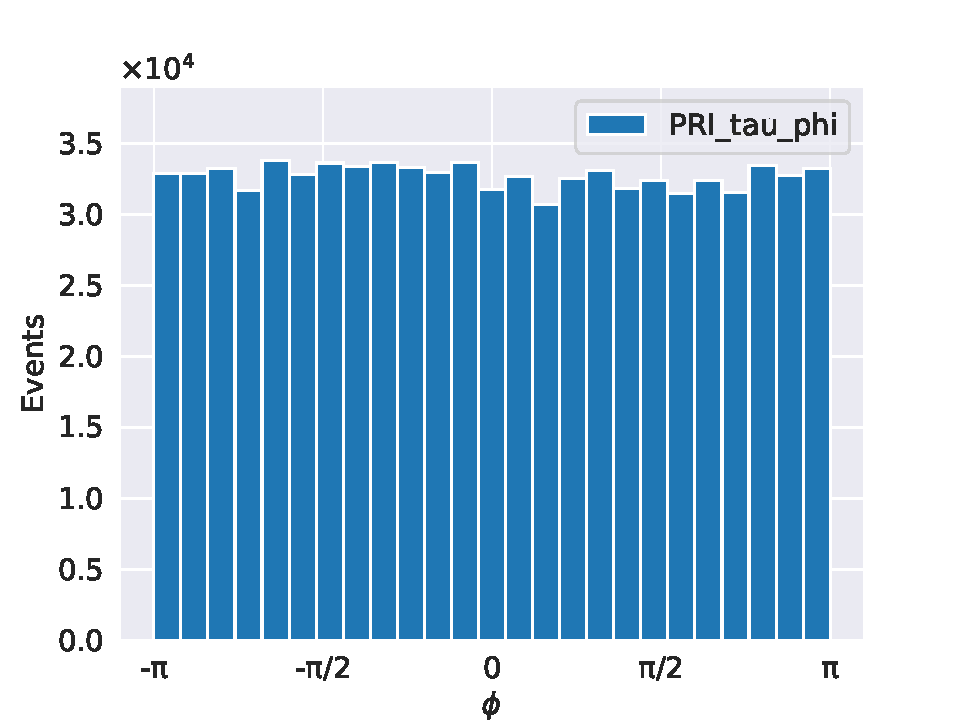
\includegraphics[width=\textwidth]{../../plots/PRI_tau_phi.pdf}
            \caption{Caption for image 1}
            \label{fig:sub1}
        \end{subfigure} &
        \begin{subfigure}[b]{0.50\textwidth}
            \centering
            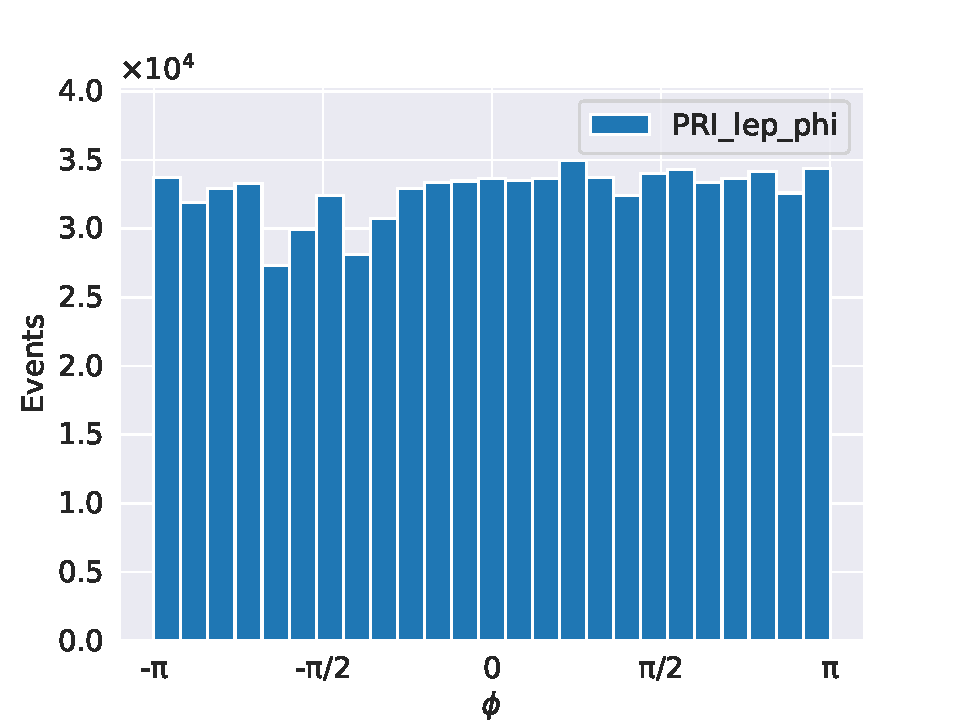
\includegraphics[width=\textwidth]{../../plots/PRI_lep_phi.pdf}
            \caption{Caption for image 2}
            \label{fig:sub2}
        \end{subfigure} \\
        \begin{subfigure}[b]{0.50\textwidth}
            \centering
            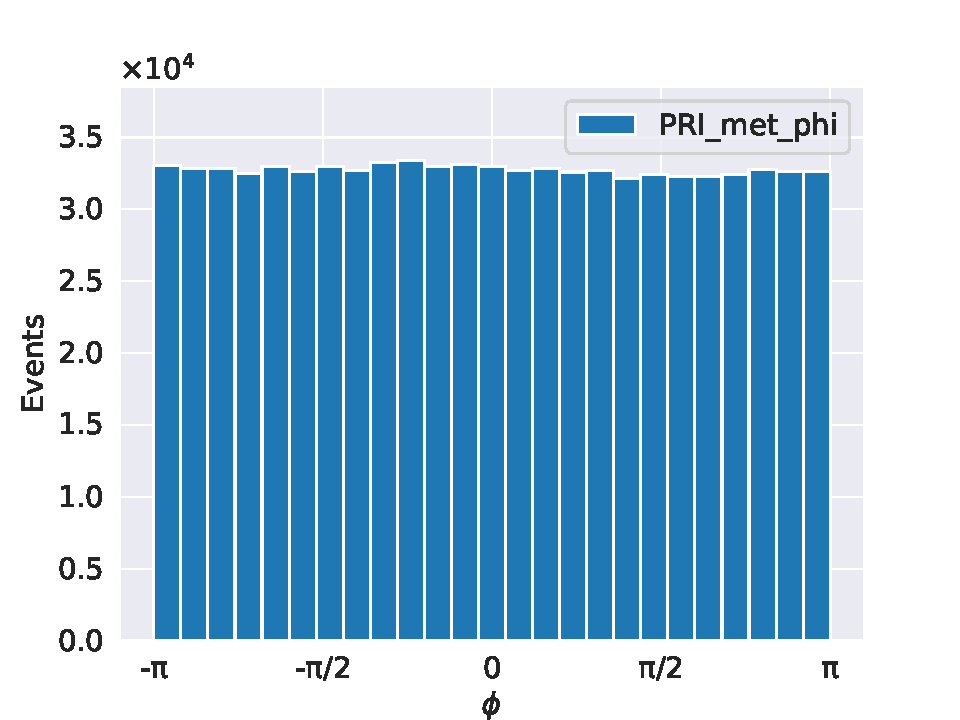
\includegraphics[width=\textwidth]{../../plots/PRI_met_phi.pdf}
            \caption{Caption for image 3}
            \label{fig:sub3}
        \end{subfigure} &
        \begin{subfigure}[b]{0.50\textwidth}
            \centering
            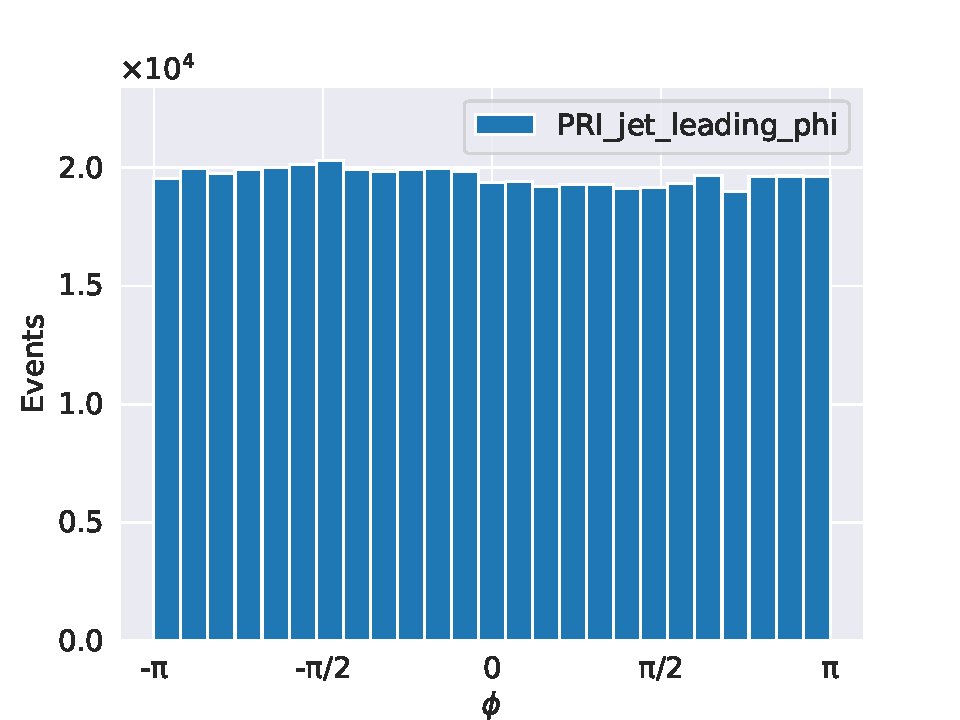
\includegraphics[width=\textwidth]{../../plots/PRI_jet_leading_phi.pdf}
            \caption{Caption for image 4}
            \label{fig:sub4}
        \end{subfigure}  \\
        \begin{subfigure}[b]{0.50\textwidth}
            \centering
            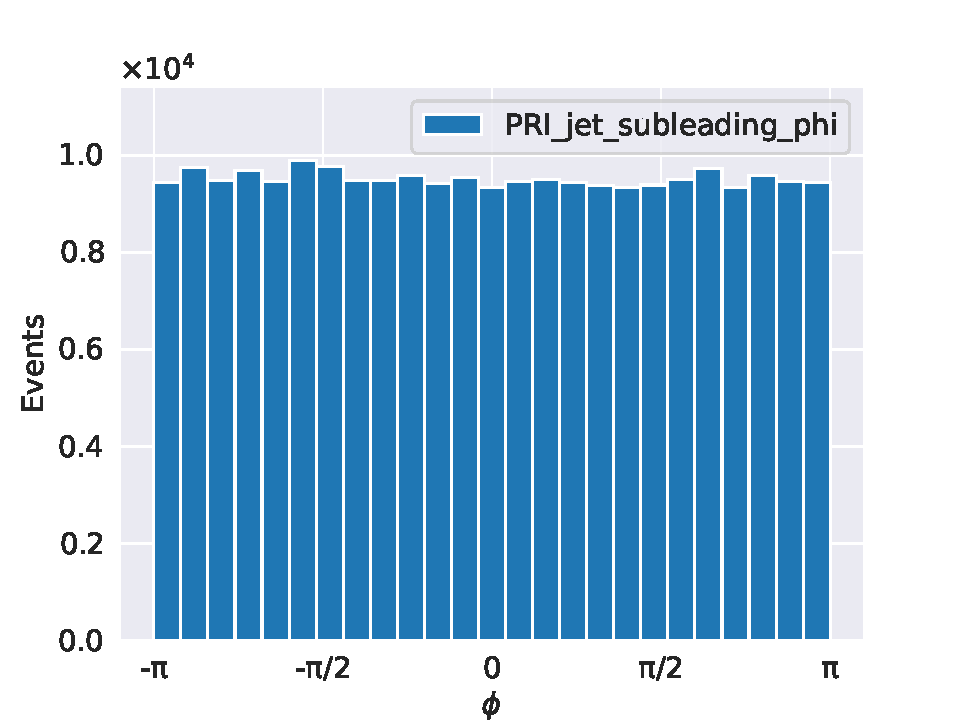
\includegraphics[width=\textwidth]{../../plots/PRI_jet_subleading_phi.pdf}
            \caption{Caption for image 4}
            \label{fig:sub4}
        \end{subfigure}
    \end{tabular}
    \caption{Main caption for the figure.}
    \label{fig:main}
\end{figure}

\end{document}


